\documentclass{article}


\usepackage[utf8]{inputenc}
\usepackage[english]{babel}
\usepackage{fancyhdr}
\usepackage{lastpage}
\usepackage{hyperref}
\usepackage{titling}
\usepackage{titlesec}
\usepackage{graphicx}
\usepackage{wrapfig}
\usepackage{listings}
%\graphicspath{ {/} }

\pagestyle{fancy}
\fancyhf{}

\lstset{basicstyle=\ttfamily,
escapeinside={||},
mathescape=true}

% last page seems to need two runs, which I assume actually means you need to create the bulid and render files in a
% certain order
% https://tex.stackexchange.com/questions/28708/why-does-pagereflastpage-give-me-rather-than-page-number-of-the-last-pag
\rfoot{\thepage \hspace{1pt} of \pageref{LastPage}}

% define subtitle command
\newcommand{\subtitle}[1]{%
	\posttitle{%
		\par\end{center}
		\begin{center}\large#1\end{center}
		\vskip0.5em}%
}

% define paragraph to be a subsubsubsection
\titleclass{\subsubsubsection}{straight}[\subsection]

\newcounter{subsubsubsection}[subsubsection]
\renewcommand\thesubsubsubsection{\thesubsubsection.\arabic{subsubsubsection}}
\renewcommand\theparagraph{\thesubsubsubsection.\arabic{paragraph}} % optional; useful if paragraphs are to be numbered

\titleformat{\subsubsubsection}
  {\normalfont\normalsize\bfseries}{\thesubsubsubsection}{1em}{}
\titlespacing*{\subsubsubsection}
{0pt}{3.25ex plus 1ex minus .2ex}{1.5ex plus .2ex}

\makeatletter
\renewcommand\paragraph{\@startsection{paragraph}{5}{\z@}%
  {3.25ex \@plus1ex \@minus.2ex}%
  {-1em}%
  {\normalfont\normalsize\bfseries}}
\renewcommand\subparagraph{\@startsection{subparagraph}{6}{\parindent}%
  {3.25ex \@plus1ex \@minus .2ex}%
  {-1em}%
  {\normalfont\normalsize\bfseries}}
\def\toclevel@subsubsubsection{4}
\def\toclevel@paragraph{5}
\def\toclevel@paragraph{6}
\def\l@subsubsubsection{\@dottedtocline{4}{7em}{4em}}
\def\l@paragraph{\@dottedtocline{5}{10em}{5em}}
\def\l@subparagraph{\@dottedtocline{6}{14em}{6em}}
\makeatother

\setcounter{secnumdepth}{4}
\setcounter{tocdepth}{4}


\title{Steem}
\subtitle{An incentivized, blockchain-based social media platform.}
\date{March 2016}
\author{
	Daniel Larimer\
	\and
	Ned Scott\
	\and
	Valentine Zavgorodnev\
	\and
	Benjamin Johnson\
	\and
	James Calfee\
	\and
	Michael Vandeberg
	}

\pagenumbering{arabic}

\begin{document}

	\renewcommand \thesection{\roman{section}}

	\maketitle

	\newpage

	\section{Abstract}

		Steem is a blockchain database that supports community building and social interaction with cryptocurrency rewards. Steem combines concepts from social media with lessons learned from building cryptocurrencies and their communities. An important key to inspiring participation in any community, currency or free market economy is a fair accounting system that consistently reflects each person's contribution. Steem is the first cryptocurrency that attempts to accurately and transparently reward an unbounded number of individuals who make \textit{subjective contributions} to its community.

	\newpage

	\section{Table of Contents}

	\tableofcontents

	\newpage

	\setcounter{section}{0}

	\renewcommand \thesection{\arabic{section}}

	\section{Introduction}

	    \paragraph{}
			Collectively, user-generated content has created billions of dollars worth of value for the shareholders of social media companies, such as Reddit, Facebook, and Twitter. \textbf{In 2014, Reddit hypothesized that its platform would be improved if everyone who contributed to reddit.com by posting stories, adding comments or voting were rewarded with a fair share in Reddit, Inc\footnote{Reddit's Cryptocurrency, Forbes, Erika Morphy, October 2014,\newline\url{http://www.forbes.com/sites/erikamorphy/2014/10/01/reddits-cryptocurrency-could-have-many-uses/\#4e07b05332b9}}}. Steem aims to support social media and online communities by returning much of its value to the people who provide valuable contributions by rewarding them with cryptocurrency, and through this process create a currency that is able to reach a broad market, including people who have yet to participate in any cryptocurrency economy.

		\paragraph{}
			There are some key principles that have been used to guide the design of Steem. The most important principle is that everyone who contributes to a venture should receive pro-rata ownership, payment or debt from the venture. This principle is the same principle that is applied to all startups as they allocate shares at founding and during subsequent funding rounds.

		\paragraph{}
			The second principle is that all forms of capital are equally valuable. This means that those who contribute their scarce time and attention toward producing and curating content for others are just as valuable as those who contribute their scarce cash. This is the sweat equity principle\footnote{Sweat Equity, Investopedia,\newline\url{http://www.investopedia.com/terms/s/sweatequity.asp}} and is a concept that prior cryptocurrencies have often had trouble providing to more than a few dozen individuals.

		\paragraph{}
			The third principle is that the community produces products to serve its members. This principle is exempli ed by credit unions, food co-ops, and health sharing plans, which serve the members of their community rather than sell products or services to people outside the community.

		\paragraph{}
			The Steem community provides the following services to its members:

		\begin{enumerate}
			\item A source of curated news and commentary.
			\item A means to get high quality answers to personalized questions.
			\item A stable cryptocurrency pegged to the U.S. dollar.
			\item Free payments.
			\item Jobs providing above services to other members.
		\end{enumerate}

		\paragraph{}
			Steem's purposeful realignment of economic incentives has the potential to produce fairer and more inclusive results for everyone involved than the social media and cryptocurrency platforms that have gone before it. This paper will explore the existing economic incentives and demonstrate how Steem's incentives may result in better outcomes for most participants.

		\subsection{Recognizing Contribution}

			\paragraph{}
				Steem is designed from the ground up to address the major barriers to adoption and monetization of a social media based economy. Our thesis is that the same techniques used to grow major social media platforms can be used to bootstrap a successful cryptocurrency. Economic incentives enabled by cryptocurrency can dramatically facilitate the growth of a new social media platform. It is the synergy between cryptocurrency and social media that we believe may give Steem a powerful advantage in the market.

			\paragraph{}
				The challenge faced by Steem is deriving an algorithm for scoring individual contributions that most community members consider to be a fair assessment of the subjective value of each contribution. In a perfect world, community members would cooperate to rate each other's contribution and derive a fair compensation. In the real world, algorithms must be designed in such a manner that they are resistant to intentional manipulation for profit. Any widespread abuse of the scoring system could cause community members to lose faith in the perceived fairness of the economic system.

			\paragraph{}
				Existing platforms operate on a one-user, one-vote principle. This creates an environment where rankings can be manipulated by sybil attacks and the service providers must pro-actively identify and block abusers. People already attempt to manipulate the Reddit, Facebook, and Twitter scoring algorithms when the only reward is web traffic or censorship.

			\paragraph{}
				The fundamental unit of account on the Steem platform is STEEM, a crypto currency token. Steem operates on the basis of one-STEEM, one-vote. Under this model, individuals who have contributed the most to the platform, as measured by their account balance, have the most influence over how contributions are scored. Furthermore, Steem only allows members to vote with STEEM when it is committed to a multi-year vesting schedule. Under this model, members have a financial incentive to vote in a way that maximises the long term value of their STEEM.

			\paragraph{}
				Steem is designed around a relatively simple concept: \textit{everyone's meaningful contribution to the community should be recognized for the value it adds.} When people are recognized for their meaningful contributions, they continue contributing and the community grows. Any imbalance in the give and take within a community is unsustainable. Eventually the givers grow tired of supporting the takers and disengage from the community.

			\paragraph{}
				The challenge is creating a system capable of identifying what contributions are needed and their relative worth in a way that can scale to an unbounded number of people.

			\paragraph{}
				A proven system for evaluating and rewarding contributions is the free market. The free market can be viewed as a single community where everyone trades with one another and rewards are allocated by profit and loss. The market system rewards those who provide value to others and punishes those who consume more value than they produce. The free market supports many different currencies and money is simply a commodity that everyone finds easy to exchange.

			\paragraph{}
				Since the free market is a proven system, it is tempting to try to create a free-market system where content consumers directly pay content producers. However, direct payment is inefficient and not really viable for content creation and curation. The value of most content is so low relative to the cognitive, financial, and opportunity costs associated with making a payment that few readers choose to tip. The abundance of free alternatives means that enforcing a 'paywall' will drive readers elsewhere. There have been several attempts to implement per-article micropayments from readers to authors, but none have become widespread.

			\paragraph{}
				Steem is designed to enable effective micropayments for all kinds of contribution by changing the economic equation. Readers no longer have to decide whether or not they want to pay someone from their own pocket, instead they can vote content up or down and Steem will use their votes to determine individual rewards. This means that people are given a familiar and widely used interface and no longer face the cognitive,  nancial, and opportunity costs associated traditional micropayment and tipping platforms.

			\paragraph{}
				Voting input from community members is critical for Steem to accurately allocate payments to contributors. Voting can therefore be viewed as a crucial contribution and worthy of rewards on its own. Some platforms, such as Slashdot, use meta-moderation\footnote{\textbf{Meta-moderation} is a second level of comment moderation. Users are invited to rate a moderator's decision in order to improve moderation.\newline\url{https://en.wikipedia.org/wiki/Meta-moderation_system}} as a way to rank and reward honest moderators. Steem chooses to reward those who contribute the most to the total promotion of a piece of content and rewards the voters proportional to the ultimate reward paid to the content creator.

			\paragraph{}
				There are other forms of contribution that Steem recognizes and rewards using objective metrics. Among these are: transaction validation, proof of work mining, liquidity rewards, and reporting of misbehaving block producers.

	\section{Ways to Contribute}

		This section outlines the ideas behind Steem and its rewards for people who provide meaningful and measurable contributions to the Steem community.

		\subsection{Capital Contributions}

			\paragraph{}
				There are two items a community can offer to attract capital: debt and ownership. Those who buy ownership profit when the community grows but lose if the community shrinks. Those who buy debt are guaranteed a certain amount of interest but do not get to participate in any profits realized by the growth of the community. Both types of capital contributions are valuable to the growth of the community and value of its currency. Additionally there are two ways ownership can be held: liquid and vesting. Vesting ownership makes a long-term commitment and cannot be sold for a minimum period of time.

			\paragraph{}
				The Steem network calls these different asset classes Steem (STEEM), Steem Power (SP), and Steem Dollars (SMD).

		\subsection{Steem (STEEM)}

			\paragraph{}
				Steem is the fundamental unit of account on the Steem blockchain. All other tokens derive their value from the value of STEEM. Generally speaking STEEM should be held for short periods of time when liquidity is needed. Someone looking to enter or exit the Steem platform will have to buy or sell STEEM. Once STEEM has been purchased it should be converted into SP or SMD to mitigate the impact of dilution over the long-term.

			\paragraph{}
				STEEM is constantly increasing in supply by 100\% per year due to non-SMD incentives. Someone who holds STEEM without converting it to SP is diluted by approximately 0.19\% per day. While the rate may appear high, for transactions that take less than 10 days, it is still cheaper than credit card processing fees. Furthermore, the daily token creation is insigni cant next to the daily volatility.

			\paragraph{}
				Someone who buys Bitcoin or any other cryptocurrency and sells it 10 days later could easily lose 3\% or more due to price fluctuations. Someone who buys Bitcoin and then sells it the same day will usually pay more than 0.4\% in market fees alone. In other words, the in ation rate is effectively insignificant during the period of time the typical individual will hold STEEM.

			\paragraph{}
				The majority of inflation is actually an accounting artifact rather than true reallocation of wealth. 90\% of non-SMD in ation is distributed back to existing holders of STEEM proportional to the STEEM value of their SP balance, making in ation more of a "split". Only about 10\% of non-SMD in ation redistributes ownership in the network.

		\subsection{Steem Power (SP)}

			\paragraph{}
				Start up companies require long-term capital commitment. Those who invest their money in a startup expect to wait years before they can sell their shares and realize their profits. Without long-term commitment, a startup seeking to raise additional capital through the sale of additional shares would be competing with existing shareholders looking to exit. Savvy investors want their capital contributions to grow the company, but growth cannot happen if the new capital is given away to those looking to exit.

			\paragraph{}
				There is significant value to having long-term commitment because it enables communities to make long-term plans. Long term commitment of stakeholders also causes them to vote for long-term growth rather than short-term pumps.

			\paragraph{}
				In the cryptocurrency space, speculators jump from cryptocurrency to cryptocurrency based mostly on which one is expected to have short-term growth. Steem wants to build a community that is mostly owned and entirely controlled by those with a long-term perspective.

			\paragraph{}
				Because Steem wants to encourage long-term growth, it is hardwired to allocate 9 STEEM to Steem Power (SP) stakeholders for every 1 STEEM it creates to fund growth through contribution incentives. Over time this drives the ratio of the total STEEM value of Steem Power balances to the total of STEEM balances toward 9:1 . (It seems likely that the ratio will be somewhat greater than 9:1 due to continued net Powering Up of the newly printed STEEM.) It also means that long-term holders are almost completely protected from the dilution used to fund growth.

			\paragraph{}
				SP can only be converted back to STEEM over 2 years via 104 equal weekly payments. '1 SP' can be viewed as a share in a pool of STEEM. The network automatically adds STEEM to the pool every block. At any time users can convert their STEEM into SP at the same ratio as STEEM in the vesting pool to total SP. Converting STEEM to SP does not dilute existing holders of SP. Likewise, every time SP is converted back to STEEM it is done at the current ratio. Individuals are guaranteed to have more STEEM in the future than they have when they  rst convert from STEEM to SP.

			\paragraph{}
				SP balances are non-transferrable and non-divisible except via the automatically recurring conversion requests. This means that SP cannot be easily traded on cryptocurrency exchanges.

			\paragraph{}
				SP is a requirement for voting for or against content. This means that SP is an access token that grants its holders exclusive powers within the Steem platform.

			\paragraph{}
				 Transferring from STEEM to SP is referred to as powering up while transferring from SP to Steem is referred to as "powering down." For example, one can power down their STEEM over a period of two years, yet one can power up their STEEM instantly.

		\subsection{Steem Dollars (SMD)}

			\paragraph{}
				Stability is an important feature of successful global economies. Without stability, individuals across the world could not have low cognitive costs while engaging in commerce and savings. Because stability is an important feature of successful economies, Steem Dollars were designed as an attempt to bring stability to the world of cryptocurrency and to the individuals who use the Steem network.

			\paragraph{}
				Steem Dollars are created by a mechanism similar to convertible notes, which are often used to fund startups. In the startup world, convertible notes are short-term debt instruments that can be converted to ownership at a rate determined in the future, typically during a future funding round. A blockchain based token can be viewed as ownership in the community whereas a convertible note can be viewed as a debt denominated in any other commodity or currency. The terms of the convertible note allow the holder to convert to the backing token with a minimum notice at the fair market price of the token. Creating token-convertible-dollars enables blockchains to grow their network effect while maximizing the return for token holders.

			\paragraph{}
				Steem Dollars are referred to with the symbol SMD, an acronym for Steem Dollars. Creating SMD requires a combination of a reliable price feed, rules to prevent abuse, and liquidity. Providing a reliable price feed involves three factors: minimizing the impact of an incorrect feed, maximizing the cost of producing an incorrect feed, and minimizing the importance of timing.

			\subsubsection{Minimizing Fraudulent Feeds}

				\paragraph{}
					SP holders elect individuals to publish price feeds. These elected individuals are presumably trusted by those who have a vested interest in the quality of the feed. By paying those who are elected, Steem creates market competition to earn the right to produce feeds. The more the feed producers are paid the more they have to lose by publishing false information.

				\paragraph{}
					Given a set of trusted and elected feed producers, the actual price used for conversions can be derived as the median of the feeds. In this way if any minority of individual feed producers produce outliers they have minimal impact on the actual median while still having the ability impact their reputation.

				\paragraph{}
					Even if all feed producers are honest, it is possible for the majority of feed producers to be impacted by events beyond their control. The Steem network is designed to tolerate short-term corruption of the median price feed while the community actively works to correct the issue. One example of an issue that may take some time to correct is short-term market manipulation. Market manipulation is difficult and expensive to maintain for long periods of time. Another example would be the failure of a centralized exchange or the corruption of the data published by the exchange.

				\paragraph{}
					Steem factors out short-term price fluctuations by using the median price over a period of one week. The median published feed is sampled every hour on the hour.

				\paragraph{}
					As long as the price feed corruption lasts for less than half the moving median time window it will have minimal impact on the conversion price. In the event the feed does get corrupted, network participants will have an opportunity to vote-out corrupt feed producers before the corrupted feed can impact the actual conversion price. Perhaps more importantly, it gives feed producers an opportunity to detect and correct issues before their feeds start impacting the price.

				\paragraph{}
					With a one week window, community members have three and a half days to respond to any issues that come up.

			\subsubsection{Mitigating Timing Attacks}

				\paragraph{}
					Market participants have access to information faster than the blockchain's one week moving median conversion price can react. This information could be used to benefit of traders at the expense of the community. If there is a sudden increase in the value of STEEM traders could request conversion of their SMD at the old, lower price, and then sell the STEEM they receive a the new higher price with minimal risk.

				\paragraph{}
					Steem levels the playing field by requiring all conversion requests to be delayed for one week. This means that neither the traders nor the blockchain has any information advantage regarding the price at the time the conversion is executed.

			\subsubsection{Minimizing Abuse of Conversions}

				\paragraph{}
					If people could freely convert in both directions then traders could take advantage of the blockchains conversion rates by trading large volumes without changing the price. Traders who see a massive run up in price would convert to SMD at the high price (when it is most risky) and then convert back after the correction. The Steem protocol protects the community from this kind of abuse by only allowing people to convert from SMD to STEEM and not the other way around.

				\paragraph{}
					The blockchain decides how and when to create SMD and who should get it. This keeps the rate of SMD creation stable and removes most avenues of abuse.

			\subsubsection{Liquidity}

				\paragraph{}
					Just because SMD can be converted to a dollars worth of STEEM at a fair price in a reasonable amount of time doesn't mean it will be viewed as a reliable dollar replacement. These assets require liquidity in a market that enables instantaneous conversion between STEEM and SMD. The measures a blockchain is forced to take to prevent abuse end up lowering the quality of the convertible dollars. To compensate for this loss of quality the blockchain can offer a  xed cost reward to liquidity providers. Whereas the potential losses from manipulation and abuse are unbounded, the cost of encouraging liquidity can be fixed.

				\paragraph{}
					A liquidity provider buys and sells SMD and STEEM. They take on the majority of the short-term price risk and long-term feed risk giving the remaining market participants a high quality, extremely liquid market within which to trade.

				\paragraph{}
					Steem has an on-blockchain market between SMD and STEEM. Users can earn rewards by providing liquidity to both sides of this market. The blockchain uses a simple algorithm to rank each user's liquidity provision and consumption.

				\paragraph{}
					A user is considered a liquidity provider if they leave an open order on the books for at least 1 minute and the order is eventually filled. If the order is canceled before being filled then the user is not credited with providing liquidity.

				\paragraph{}
					Users must provide liquidity on both sides of the book to qualify for rewards and they must provide liquidity consistently over time. The scoring algorithm is:

				\begin{lstlisting}
	LiquidityPoints = NetBidVolume x NetAskVolume
				\end{lstlisting}

				\paragraph{}
					Every hour the account with the most LiquidityPoints receives 1200 STEEM and then has its LiquidityPoints reset to 0. An account that goes a week without earning any LiquidityPoints also has its points reset to 0. This means that whether you provide a large amount of liquidity or a small amount over a long period of time everyone gets a proportional amount of the rewards. If either NetBidVolume or NetAskVolume is negative, then LiquidityPoints is considered to be 0.

			\subsubsection{Sustainable Debt to Ownership Ratios}

				\paragraph{}
					If a token is viewed as ownership in the whole supply of tokens, then a token-convertible-dollar can be viewed as debt. If the debt to ownership ratio gets too high the entire currency can become unstable. Debt conversions can dramatically increase the token supply, which in turn is sold on the market suppressing the price. Subsequent conversions require the issuance of even more tokens. Left unchecked the system can collapse leaving worthless ownership backing a mountain of debt. The higher the debt to ownership ratio becomes the less willing new investors are to bring capital to the table.

				\paragraph{}
					For every SMD Steem creates, \$19.00 of STEEM is also created and converted to SP. This means that the highest possible debt-to-ownership in a stable market is 1:19 or about 5\%. If Steem falls in value by 50\% then the ratio could increase to 10\%. An 88\% fall in value of STEEM could cause the debt-to-ownership ratio to reach 40\%. Assuming the value of STEEM eventually stabilizes, the debt-to-ownership ratio will naturally move back toward 5\%.

				\paragraph{}
					The idea behind having a conservative 5\% debt to ownership ratio is that even if all debt were converted and sold there should be ample buyers and the effective dilution of the token holders remains relatively small.

				\paragraph{}
					A rapid change in the value of STEEM can dramatically change the debt-to-ownership ratio. The percentage floors used to compute STEEM creation are based on the supply including the STEEM value of all outstanding SMD and SP (as determined by the current rate / feed).

			\subsubsection{Interest}

				\paragraph{}
					SMD pays holders interest. The interest rate is set by the same people who publish the price feed so that it can adapt to changing market conditions. All debt carries risk to the lender. Someone who holds SMD without redeeming it is effectively lending the community the value of a dollar. They are trusting that at some point in the future someone will be willing to buy the SMD from them for a dollar or that there will be speculators and investors willing to buy the STEEM they convert it into.

				\paragraph{}
					STEEM and SP holders gain leverage when members of the community are willing to hold SMD. This leverage amplifies the gains from growth while also contributing to growth. STEEM holders do suffer from increased dilution if the price falls. Cryptocurrency projects have shown that the gains from increasing the user base willing to trust the network with capital ultimately add more value to the network than any dilution that may occur during a downturn.

			\subsubsection{Setting Price Feeds}

				\paragraph{}
					Astute readers will recognize that an interest bearing asset of limited supply may trade higher or lower than the underlying asset depending upon other opportunities to earn interest on the same asset. With a high interest rate paid on an asset pegged to the US dollar many people will bid up the limited supply of Steem Dollars until they are no longer valued at \$1. In economics there is a principle known as the Impossible Trinity\footnote{The Impossible Trinity, economic theory\newline\url{https://en.wikipedia.org/wiki/Impossible_trinity}} which states that it is impossible to have all three of the following at the same time:

				\begin{enumerate}
					\item A stable exchange rate
					\item Free capital movement
					\item An independent monetary policy
				\end{enumerate}

				\paragraph{}
					If Steem feed producers aim to have an independent monetary policy allowing it to create and destroy Steem Dollars while simultaneously having full control over the interest rate then they will encounter problems. The Impossible Trinity says that Steem Dollars either need to restrict capital movement, have an unstable exchange rate with the dollar, or have limited control over the interest rate.

				\paragraph{}
					The primary concern of Steem feed producers is to maintain a stable one-to-one conversion between SMD and the U.S. Dollar (USD). Any time SMD is consistently trading above \$1.00 USD interest payments must be stopped. In a market where 0\% interest on debt still demands a premium, it is safe to say the market is willing to extend more credit than the debt the community is willing to take on. If this happens a SMD will be valued at more than \$1.00 and there is little the community can do without charging negative interest rates.

				\paragraph{}
					If the debt-to-ownership ratio is under 10\% and SMD is trading for less than \$1.00 then the interest rate should be increased. This will encourage more people to hold their SMD and support the price.

				\paragraph{}
					If SMD trades for less than \$1.00 USD and the debt-to-ownership ratio is over 10\% then the feeds should be adjusted upward give more STEEM per SMD. This will increase demand for SMD while also reducing the debt-to-ownership ratio and returning SMD to parity with USD.

				\paragraph{}
					Assuming the value of STEEM is growing faster than Steem is creating new SMD, the debt-to-ownership ratio should remain under the target ratio and the interest offered bene ts everyone. If the value of the network is  at or falling, then any interest offered will only make the debt-to-ownership ratio worse.

				\paragraph{}
					In effect, feed producers are entrusted with the responsibility of setting monetary policy for the purpose of maintaining a stable peg to the USD. Abuse of this power can harm the value of STEEM so SP holders are wise to vote for witnesses that can be counted on to adjust the price feed and interest rates according to the rules outlined above.

				\paragraph{}
					If the debt-to-ownership ratio gets dangerously high and market participants choose to avoid conversion requests, then the feed should be adjusted to increase the rate at which STEEM paid for converting SMD.

				\paragraph{}
					Changes to the interest rate policy and/or any premiums/discounts on the STEEM/SMD conversion rate should be a slow and measured response to long-term average deviations rather than attempting to respond to short-term market conditions. The blockchain is paying liquidity providers for their service in absorbing short-term demands.

				\paragraph{}
					It is our belief that these rules will give market participants con dence that they are unlikely lose money by holding SMD purchased at a price of \$1.00. We fully expect there to be a narrow trading range between \$0.99 and \$1.01 for SMD under most market conditions.

		\subsection{Subjective Contributions}

			\paragraph{}
				Subjective Proof of Work presents an alternative approach to distributing a currency that improves upon fully \textit{objective} Proof of Work systems such as mining. The applications of a currency implementing \textit{subjective} proof of work are far wider than any \textit{objective} proof of work system because they can be applied to build a community around any concept that has a sufficiently de ned purpose. When individuals join a community they buy into a particular set of beliefs and can vote to reinforce the community values or purpose.

			\paragraph{}
				In effect, the criteria by which work is evaluated is completely subjective and its definition lives outside the source code itself. One community may wish to reward artists, another poets, and another comedians. Other communities may choose to reward charitable causes or help advance political agendas.

			\paragraph{}
				The value each currency achieves depends upon the demand for in uence within a particular community and how large the market believes each community can get. Unlike prior systems, subjective proof of work enables a community to collectively fund the development of whatever it finds valuable and enables the monetization of previously non monetizable time.

			\subsubsection{Distributing Currency}

				\paragraph{}
					There are two ways people can get involved with a crypto-currency community: they can \textit{buy in}, or they can \textit{work in}. In both cases users are adding value to the currency, however, the vast majority of people have more \textit{free time} than they do \textit{spare cash}. Imagine the goal of bootstrapping a currency in a poor community with no actual \textit{cash} but plenty of \textit{time}. If people can earn money by working for one another then they will bootstrap value through mutual exchange facilitated by a fair accounting/currency system.

				\paragraph{}
					Distributing a currency to as many people as possible in a manner that is generally perceived as fair is a challenging task. The tasks that can be entirely evaluated by an objective computer algorithm are limited in nature and generally speaking have limited positive external benefits. In the case of Bitcoin-style mining, it can result in the production of specialized hardware and cause people to invest time developing more ef cient algorithms. It may even help find prime numbers, but none of these things provide meaningful value to society or the currency holding community at large. More importantly, economies of scale and market forces will end up excluding everyone but experts from participating in this kind of distribution. Ultimately, computation-based mining is just another way of \textit{buying} in because it requires money to pay the electric bill or the development of hardware necessary to do the work.

				\paragraph{}
					In order to give everyone an equal opportunity to get involved and earn the currency people must be given an opportunity to work. The challenge is how to judge the relative quality and quantity of work that individuals provide and to do so in a way that ef ciently allocates rewards to millions of users. This requires the introduction of a scalable voting process. In particular it requires that authority to allocate funds must be as distributed and decentralized as possible.

				\paragraph{}
					The first step in rewarding millions of users is to commit to distributing a fixed amount of currency regardless of how much work is actually done or how users vote. This changes the question from being \textit{"Should we pay?"} to \textit{"Whom should we pay?"} and signals to the market that money is being distributed and is being auctioned off to whoever "bids" the most \textit{work}. This is similar to Bitcoin committing to award 50 BTC to whoever finds the most difficult hashes. Like Bitcoin, all work must be done prior-to payout and nothing should be paid speculatively on the promise to do work in the future.

				\paragraph{}
					The next step is to reward everyone who does anything even remotely positive with \textit{something}. This is accomplished by ranking all work done and distributing proportionally to its value. The more competitive the market becomes, the more difficult (higher quality or quantity) it becomes to earn the same payout.

			\subsubsection{Voting on Distribution of Currency}

				\paragraph{}
					Assume there is a fixed amount of money to distribute, and that those who have a long-term vested interest in the future value and utility of the currency are the ones who must decide how to allocate it. Every vesting user casts their votes on who did the best work and at the end of the day the available money for that day is divided proportional to the votes such that everyone with even one net positive vote gets something.

				\paragraph{}
					The naive voting process creates a Prisoner's Dilemma whereby each individual voter has incentive to vote for themselves at the expense of the larger community goal. If every voter defects by voting for themselves then no currency will end up distributed and the currency as a whole will fail to gain network effect. On the other hand, if only one voter defects then that voter would win undeserved profits while having minimal effect on the overall value of the currency.

				\paragraph{}
					In order to realign incentives and discourage individuals from simply voting for themselves, money must be distributed in a nonlinear manner. For example a quadratic function in votes, i.e., someone with twice the votes of someone else should receive four times the payout and someone with three times the votes should receive nine times the payout. In other words, the reward is proportional to votes2 rather than votes. This mirrors the value of network effect which grows with n2 the number of participants, according to Metcalfe's Law\footnote{Metcalfe's Law\url{https://en.wikipedia.org/wiki/Metcalfe\%27s_law}}.

				\paragraph{}
					Assuming all users have equal stake, someone who only receives their own vote will receive much less than someone who receives votes from 100 different users. This encourages users to \textit{cooperate} to vote for the same things to maximize the payout. This system also creates financial incentive to \textit{collude} where everyone votes on one thing and then divides the reward equally among themselves.

				\subsubsubsection{Voting Collusion}

					\paragraph{}
						While cooperation to distribute funds to the best work is the desired goal, collusion that undermines this objective should be minimized. There are two kinds of collusion, the most straightforward is when one user simply buys a larger stake than others, and the other involves coordinating a large number of smaller stakeholders to work together. Larger stakeholders can have the voting influence of 100 or even 1000 smaller stakeholders which means they have even greater incentive to defect by voting for themselves than they had under a linear distribution.

					\paragraph{}

						Regardless of how much money any one individual has, there are always many other individuals with similar wealth. Even the wealthiest individual rarely has much more than the next couple wealthiest combined. Furthermore, those who have a large investment in a community also have the most to lose by attempting to game the voting system for themselves. It would be like the CEO of a company deciding to stop paying salaries so he could pocket all of the profits. Everyone would leave to work for other companies and the company would become worthless, leaving the CEO bankrupt rather than wealthy.

					\paragraph{}
						Fortunately, any work that is getting a large concentration of votes is also gaining the most scrutiny (publicity). Through the addition of negative-voting it is possible for many smaller stakeholders to nullify the voting power of collusive groups or defecting large stakeholders. Furthermore, large-stakeholders have more to lose if the currency falls in value due to abuse than they might gain by voting for themselves. In fact, honest large stakeholders are likely to be more effective by policing abuse and using negative voting than they would be by voting for smaller contributions.

					\paragraph{}
						The use of negative-voting to keep people from abusing the system leverages the crab mentality that many people have when it is perceived that one individual is pro ting at the expense of everyone else. While crab mentality normally refers to short-sighted people keeping good people down, it is also what allows good people to keep bad people down. The only "problem" with crab mentality is when people wrongly believe someone is profiting at everyone else's expense.

				\begin{quote}

				\subsubsubsection[The Story of the Crab Bucket]{The Story of the Crab Bucket\protect\footnote{The Story of the Crab Bucket, \url{http://guidezone.e-guiding.com/jmstory_crabs.htm}}}

					\paragraph{}
						A man was walking along the beach and saw another man  shing in the surf with a bait bucket beside him. As he drew closer, he saw that the bait bucket had no lid and had live crabs inside.

					\paragraph{}
						"Why don't you cover your bait bucket so the crabs won't escape?", he said.

					\paragraph{}
						"You don't understand.", the man replied, "If there is one crab in the bucket it would surely crawl out very quickly. However, when there are many crabs in the bucket, if one tries to crawl up the side, the others grab hold of it and pull it back down so that it will share the same fate as the rest of them."

					\paragraph{}
						So it is with people. If one tries to do something different, get better grades, improve herself, escape her environment, or dream big dreams, other people will try to drag her back down to share their fate.

					\end{quote}

					\paragraph{}
						Eliminating "abuse" is not possible and shouldn't be the goal. Even those who are attempting to "abuse" the system are still doing work. Any compensation they get for their successful attempts at abuse or collusion is at least as valuable for the purpose of distributing the currency as the make-work system employed by traditional Bitcoin mining or the collusive mining done via mining pools. All that is necessary is to ensure that abuse isn't so rampant that it undermines the incentive to do real work in support of the community and its currency.

					\paragraph{}
						The goal of building a community currency is to get more "crabs in the bucket". Going to extreme measures to eliminate all abuse is like attempting to put a lid on the bucket to prevent a few crabs from escaping and comes at the expense of making it harder to add new crabs to the bucket. It is sufficient to make the walls slippery and give the other crabs suf cient power to prevent others from escaping.

			\subsubsection{Rate Limited Voting}

				\paragraph{}
					A major part of minimizing abuse is the rate-limiting of voting. Individual users can only read and evaluate so many work items per day. Any attempt to vote more frequently than this is a sign of automation and potential abuse. Through rate limiting, stakeholders who vote more frequently have each vote count for less than stakeholders who vote less frequently. Attempts to divide tokens among multiple accounts also divides in uence and therefore does not result in a net increase in in uence nor bypass the rate-limit imposed on voting.

				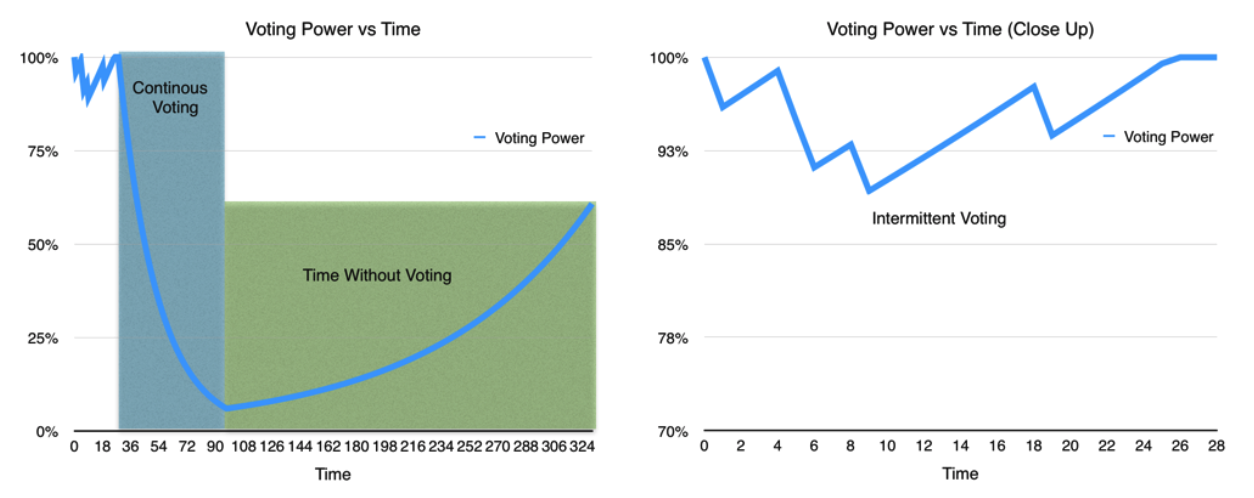
\includegraphics[width=11cm]{img_voting_rate_limiting}

				\paragraph{}
					The charts above shows how a user's voting power decreases every time they vote and then regenerates as time passes without voting. These charts use nominal time unit and could be made to scale to any targeted voting rate. Note that voting power rapidly drops off during periods of continuous voting, and then slowly recovers.
				
				\paragraph{}
					Voting power is multiplied by a user's vesting tokens to determine how much share in the reward pool should be allocated to a given work item.

			\subsubsection{Delayed Payouts}

				\begin{wrapfigure}{r}{0.5\textwidth}
                    \centering
                    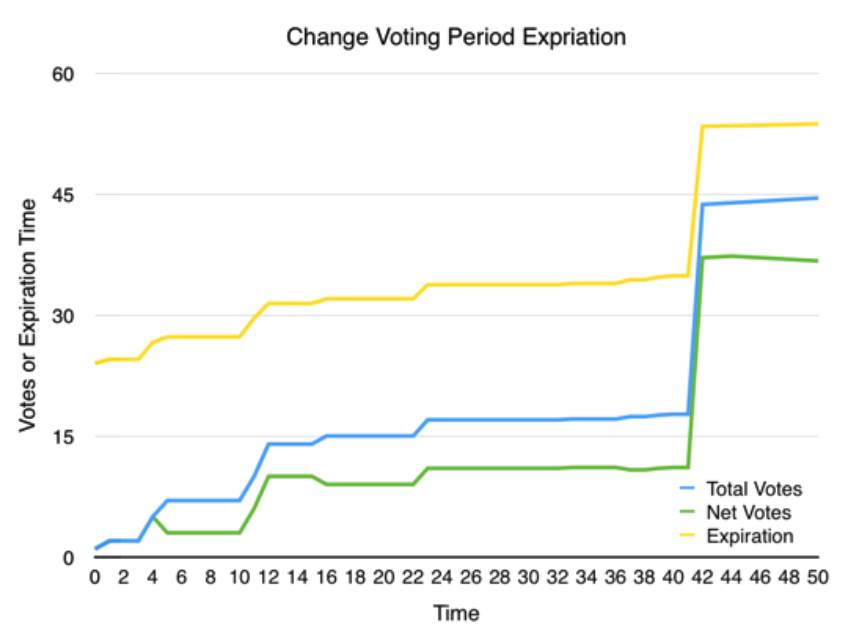
\includegraphics[width=0.5\textwidth]{img_change_voting_period_eg}
                \end{wrapfigure}

				\paragraph{}
					To further prevent abuse, all payouts are delayed a stake-weighted average of 24 hours from the time each vote was cast. This ensures that large stakeholders cannot snipe payouts by voting at the last second before other voters (aka crabs) have a chance to negate the potential abuse. Once a payout is made to the user all votes are reset to 0. If votes come in after the payout then the process begins again.

				\paragraph{}
					This chart shows how the voting period expiration changes in response to new positive and negative votes being applied. New votes extend the payout period in proportion to how large they are relative to all votes that have gone before. Around time 40 a large number of new votes were added which extended the voting period by 12 hours, subsequent smaller votes had far less impact on the voting period.

			\subsubsection{Payout Distribution}

				\begin{wrapfigure}{r}{0.5\textwidth}
					\centering
					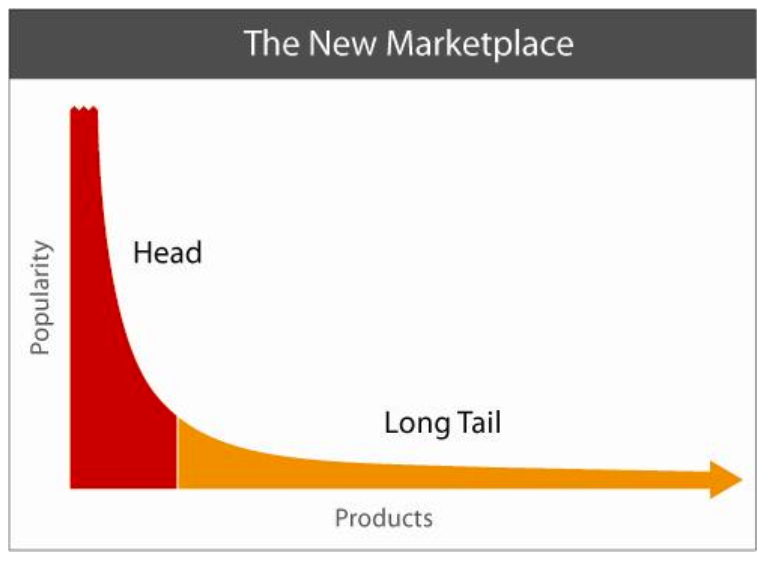
\includegraphics[width=0.5\textwidth]{img_the_new_marketplace}
				\end{wrapfigure}

				\paragraph{}
					One of the primary goals of Steem's reward system is to produce the best discussions on the internet. Each and every year 10\% of the market capitalization of Steem is distributed to users submitting, voting on, and discussing content. At the size of Bitcoin this could be as much as \$1.75 million dollars per day being given to top contributors.

				\paragraph{}
					The actual distribution will depend upon the voting patterns of users, but we suspect that the vast majority of the rewards will be distributed to the most popular content. Steem weighs payouts proportional to n2 the amount of Steem Power voting for a post. In other words, post x would receive a payout proportional to:

				\begin{lstlisting}
		votes[x$]^{2}$ / sum(votes[0...n]$^{2}$)
                \end{lstlisting}

                \paragraph{}
                	Zipf's Law\footnote{Zipf's Law \url{https://en.wikipedia.org/wiki/Zipf\%27s_law}} is one of those empirical rules that characterize a surprising range of real-world phenomena remarkably well. It says that if we order some large collection by size or popularity, the second element in the collection will be about half the measure of the first one, the third one will be about one-third the measure of the first one, and so on. In general, the $k^{th}$-ranked item will measure about 1/k of the first one.

                \paragraph{}
                	Taking popularity as a rough measure of value, then the value of each individual item is given by Zipf’s Law. That is, if we have a million items, then the most popular 100 will contribute a third of the total value, the next 10,000 another third, and the remaining 989,900 the  nal third. The value of the collection of n items is proportional to log( n ).

                \paragraph{}
                	The impact of this voting and payout distribution is to offer large bounties for good content while still rewarding smaller players for their long-tail contribution.

                \paragraph{}
                	The economic effect of this is similar to a lottery where people over-estimate their probability of getting votes and thus do more work than the expected value of their reward and thereby maximize the total amount of work performed in service of the community. The fact that everyone “wins something” plays on the same psychology that casinos use to keep people gambling. In other words, small rewards help reinforce the idea that it is possible to earn bigger rewards.

				\subsubsubsection{Rewarding Parent Posts}

					\paragraph{}
						Good discussion requires back and forth posting. When you reply to someone else, they get 50\% of any payout you receive in that thread. This rule applies up to 6 levels deep. Starting a big discussion greatly rewards the parent poster.

					\paragraph{}
						Failure to properly nest your posts in the discussion is a good way to get down voted.

					\paragraph{}
						This incentive structure motivates people to contribute in a way that motivates others to get involved. It encourages people to ask good questions so that others can provide valuable answers.
			\subsubsection{Payouts}

				\paragraph{}
					When a post receives a payout it takes the form of 50\% SMD and 50\% SP. The Steem Power give the user increased voting and transaction power while the SMD gives the user an immediate benefit in a stable currency. As we’ve already discussed at length, both SP and SMD are designed to encourage long-term holding rather than short-term selling.

	\section{Consensus Algorithm}

		\paragraph{}
			Consensus is the process by which a community comes to a universally recognized, unambiguous agreement on piece of information. There are many algorithms society has developed for reaching consensus about who owns what. Every government on earth is a primitive consensus algorithm whereby the population agrees to abide by a certain set of rules enshrined in a constitution. Governments establish courts, judges, and juries to interpret the subjective facts and render a final decision. Most of the time people abide by the decision even if it was wrong.

		\paragraph{}
			The algorithms used by cryptocurrencies provide a better way to reach consensus. Cryptographically signed testimony from individuals is recorded in a public ledger that establishes the absolute global order of events. A deterministic computer algorithm can then process this ledger to derive a universally accepted conclusion. So long as the members of a community agree on the processing algorithm, the result of the algorithm is authoritative.

		\paragraph{}
			The primary consideration is determining what testimony is allowed to enter the public record. Systems should be designed to minimize the potential for censorship. Censorship on the public ledger is similar to preventing someone from voting in an election. In both cases an individual is prevented from impacting the global consensus.

		\subsection{Consensus in Steem}

			\paragraph{}
				Conceptually, the consensus algorithm adopted by Steem is similar to the consensus algorithm adopted by companies throughout the world. People with a vested interest in the future value of Steem vote to select individuals responsible for including testimony in the public record. Voting is weighted proportional to each individual's vested interest.

			\paragraph{}
				In the world of cryptocurrencies, the public record is commonly referred to as a \textit{blockchain}. A \textit{block} is a group of signed transactions.

			\paragraph{}
				With Steem, block production is done in rounds. Each round 21 witnesses are selected to create and sign blocks of transactions. Nineteen (19) of these witnesses are selected by approval voting, one is selected by a computational proof-of-work, and one is timeshared by every witness that didn’t make it into the top 19 proportional to their total votes. The 21 active witnesses are shuffled every round to prevent any one witness from constantly ignoring blocks produced by the same witness placed before.

			\paragraph{}
				This process is designed to provide the best reliability while ensuring that everyone has the potential to participate in block production regardless of whether they are popular enough to get voted to the top. People have three options to overcome censorship by the top 19 elected witnesses: patiently wait in line with everyone else not in the top 19, purchase enough computational power to solve a proof of work faster than others, or purchase more SP to improve voting power. Generally speaking, applying censorship is a good way for elected witnesses to lose their job and therefore, it is unlikely to be a real problem on the Steem network.

			\paragraph{}
				Because the active witnesses are known in advance, Steem is able to schedule witnesses to produce blocks every 3 seconds. Witnesses synchronize their block production via the NTP protocol. A variation of this algorithm has been in use by the BitShares network for over a year where it has been proven to be reliable.

		\subsection{Mining in Steem}

			\paragraph{}
				Traditional proof of work blockchains combine block production with the solving of a proof of work. Because the process of solving a proof of work takes an unpredictable amount of time, the result is unpredictable block production times. Steem aims to have consistent and reliable block production every 3 seconds with almost no potential for forks.

			\paragraph{}
				To achieve this Steem separates block production from solving of proof of work. When a miner solves a proof of work for Steem, they broadcast a transaction containing the work. The next scheduled witness includes the transaction into the blockchain. When the transaction is included the miner is added to the queue of miners scheduled to produce blocks. Each round one miner is popped from the queue and included in the active set of witnesses. The miner gets paid when they produce a block at the time they are scheduled.

			\paragraph{}
				The difficulty of the proof of work doubles every time the queue length grows by 4. Because one miner is popped from the queue every round, and each round takes 21 * 3 = 63 seconds, the dif culty automatically halves if no proof of work is found in no more than 21 * 3 * 4 = 252 seconds.

			\subsubsection{Mining Rewards require Steem Power}

				\paragraph{}

				\paragraph{}

			\subsubsection{Mining Algorithm}

				\paragraph{}

				\paragraph{}

				%\begin{lstlisting}
				%\end{lstlisting}

			\subsubsection{Botnet Resistant}

				\paragraph{}

				\paragraph{}

				\paragraph{}

				\paragraph{}

				\paragraph{}

			\subsubsection{Mining Pool Resistant}

				\paragraph{}

				\paragraph{}

	\section{Eliminating Transaction Fees}

		\paragraph{}

		\paragraph{}

		\subsection{The Problem With Fees}

			\paragraph{}

			\paragraph{}

			\subsubsection{Micropayments Don’t Work}

				\paragraph{}

				\paragraph{}

				\begin{quote}

					\paragraph{}

					\paragraph{}

					\paragraph{}

				\end{quote}

				\paragraph{}

				\paragraph{}

			\subsubsection{Fees are a Barrier to Entry}

				\paragraph{}

			\subsubsection{Changing Fees}

				\paragraph{}

			\subsubsection{Sybil Attacks}

				\paragraph{}

				\paragraph{}

			\subsubsection{Full Reserve vs Fractional Reserve}

				\paragraph{}

				\paragraph{}

				\paragraph{}

		%Note, this sub section is missing from the original doc contents
		\subsection{Bandwidth Instead of Micropayment Channels}

			\paragraph{}

			\paragraph{}

			\paragraph{}

			\subsubsection{Example Implementation}

				\paragraph{}

				%\begin{lstlisting}
				%\end{lstlisting}

				\paragraph{}

				%\begin{lstlisting}
				%\end{lstlisting}

				\paragraph{}

				\paragraph{}

				\paragraph{}

			\subsubsection{Case Study: Bitcoin}

				\paragraph{}

				%\begin{lstlisting}
				%\end{lstlisting}

				\paragraph{}

				% TOOD : insert extra spacing or horizontal rule

				\paragraph{}

				\subsubsubsection{Impact of Capacity}

					\paragraph{}

				\subsubsubsection{Maximum Number of Unique Users}

					\paragraph{}

				\subsubsubsection{Comparison to Fees}

					\paragraph{}

			\subsubsection{Account Creation}

				\paragraph{}

				\paragraph{}

				\paragraph{}

				\paragraph{}

			\subsubsection{Justifying Minimum Balances}

				\paragraph{}

				\paragraph{}

				\paragraph{}

				\paragraph{}

				\paragraph{}

				\paragraph{}

			\subsubsection{Adjusting the Reserve Ratio}

				\paragraph{}

				\paragraph{}

				\paragraph{}

				\paragraph{}

				\paragraph{}

				\paragraph{}

			\subsubsection{Effectiveness Relative to Fees}

				\paragraph{}

				\paragraph{}

				\paragraph{}

			\subsubsection{Renting vs. Buying vs. Time Sharing}

				\paragraph{}

				\paragraph{}

				\paragraph{}

				\paragraph{}

				\paragraph{}

				\paragraph{}

				\paragraph{}

				\paragraph{}

				\paragraph{}

	\section{Performance and Scalability}

		\paragraph{}

		\subsection{Reddit Scale}

			\paragraph{}

			\paragraph{}

			%\begin{enumerate}
			%\end{enumerate}

			\paragraph{}

			\paragraph{}

	\section{Allocation & Supply}

		\paragraph{}

		\paragraph{}

		%\begin{itemize}
		%\end{itemize}

		\paragraph{}

		%\begin{itemize}
		%\end{itemize}

		\paragraph{}

		%\begin{itemize}
		%\end{itemize}

		\paragraph{}

		\paragraph{}

		\paragraph{}

		\subsection{Impact of Token Creation Rate}

			\paragraph{}

			\paragraph{}

			\paragraph{}

			\paragraph{}

			\paragraph{}

			\paragraph{}

			\paragraph{}

			\paragraph{}

			\paragraph{}

			\subsubsection{Impact of Token Creation Rate Greater than Ninety-Percent}

				\paragraph{}

				\paragraph{}

			\subsubsection{Accounting In Steem}

				\paragraph{}

				\paragraph{}

				\paragraph{}

				\paragraph{}

	\section{The Power of Steem}

		\paragraph{}

		\paragraph{}

		\paragraph{}

		\subsection{No Micropayments, Tips Optional}

			\paragraph{}

			\paragraph{}

			\paragraph{}

			\paragraph{}

			%\begin{quote}

				\paragraph{}

				\paragraph{}

			%\end{quote}

			\paragraph{}

			\paragraph{}

		\subsection{Value is in the Links}

			\paragraph{}

			\paragraph{}

			\paragraph{}

			\paragraph{}

		\subsection{Solving the Cryptocurrency Onboarding Problem}

			\paragraph{}

			\paragraph{}

		\subsection{Solving the Cryptocurrency Liquidation Problem}

			\paragraph{}

			\paragraph{}

			\paragraph{}

			\paragraph{}

		\subsection{Censorship}

			\paragraph{}

			\paragraph{}

			\paragraph{}

		\subsection{Solving Organic Discovery via Search Engine Optimization}

			\paragraph{}

		\subsection{Shifting Toward Blockchain-based Attribution}

			\paragraph{}

			\paragraph{}

			\paragraph{}

		\subsection{Replacing Advertising with Blockchain-based Content Rewards}

			\paragraph{}

			\paragraph{}

	\section{Conclusion}

\end{document}